\documentclass[11pt]{article}
\usepackage{fullpage,fourier,euler,amsmath,graphicx,xspace}
\usepackage{epigraph}
\usepackage{tcolorbox}
\usepackage{listings,color,url,hyperref}

\title{Assignment 2 \\ A Small Numerical Library}
\author{Prof. Darrell Long \\
CSE 13S -- Winter 2020}
\date{Due: January 26$^\text{th}$ at 11:59\,pm}


\usepackage{fancyhdr}
\pagestyle{fancy}
\fancyhf{}

\fancypagestyle{plain}{%
  \fancyhf{}
  \renewcommand{\headrulewidth}{0pt}
  \renewcommand{\footrulewidth}{0pt}
  \lfoot{\textcopyright{} 2021 Darrell Long}
  \rfoot{\thepage}
}

\pagestyle{plain}

\definecolor{codegreen}{rgb}{0,0.5,0}
\definecolor{codegray}{rgb}{0.5,0.5,0.5}
\definecolor{codepurple}{rgb}{0.58,0,0.82}

\lstloadlanguages{C,make,python,fortran}

\lstdefinestyle{c99}{
    morekeywords={bool, uint8_t, uint16_t, uint32_t, uint64_t, int8_t, int16_t, int32_t, int64_t},
    commentstyle=\color{codegreen},
    keywordstyle=\color{magenta},
    numberstyle=\tiny\color{codegray},
    identifierstyle=\color{blue},
    stringstyle=\color{codepurple},
    basicstyle=\ttfamily,
    breakatwhitespace=false,
    breaklines=true,
    captionpos=b,
    keepspaces=true,
    numbers=left,
    numbersep=5pt,
    showspaces=false,
    showstringspaces=false,
    showtabs=false,
    tabsize=4
}

\lstset{language=C, style=c99}
\newtcolorbox{prelab}[1]{colback=red!5!white, colframe=red!75!black, title=#1}

\begin{document}\maketitle

\section{Introduction}
\epigraphwidth=0.6\textwidth
\epigraph{\emph{Just look at the graceful way that he lectures, one hand
waves while the other conjectures.}}

\noindent As we know, computers are simple machines that carry out a sequence
of very simple steps, albeit very quickly.  Unless you have a
special-purpose processor, a computer can only compute \emph{addition},
\emph{subtraction}, \emph{multiplication}, and \emph{division}.  If you think about it,
you will see that the functions that might interest you when dealing
with real or complex numbers can be built up from those four operations.
We use many of these functions in nearly every program that we write, so we ought
to understand how they are created.

If you recall from your calculus class, with some
conditions a function $f(x)$ can be represented by its Taylor
series expansion near some point $f(a)$:
$$
f(x) = f(a) + \sum_{k=1}^\infty \frac{(x-a)^k}{k!} f^{(k)}(a) .
$$
If you have forgotten (or never taken) calculus, do not despair. Go to a
laboratory section for review: the concepts required for this assignment are just
derivatives.

Since we cannot compute an infinite series, we must be content to
calculate a
finite number of terms. In general, the more terms that we compute, the more
accurate our approximation. For example, if we expand to $10$ terms
we get:
\begin{align*}
f(x) =  f(a) & +(x-a) f'(a)+\frac{1}{2} (x-a)^2 f''(a)+\frac{1}{6} f^{(3)}(a) (x-a)^3 \\
& + \frac{1}{24}
   f^{(4)}(a) (x-a)^4+\frac{1}{120} f^{(5)}(a) (x-a)^5+\frac{1}{720} f^{(6)}(a)
   (x-a)^6 \\
& +\frac{f^{(7)}(a) (x-a)^7}{5040}+\frac{f^{(8)}(a)
   (x-a)^8}{40320}+\frac{f^{(9)}(a) (x-a)^9}{362880}
   +O\left((x-a)^{10}\right) .
\end{align*}

Taylor series, named after Brook Taylor, requires that we pick a point $a$ where we will center the approximation. In the case $a =0$, then it is called a \emph{Maclaurin series}).  Often we
choose $0$, but the closer to the value of $x$ the better we will
approximate the function. For example, let's consider $e^x$ centered
around $0$:
$$
e^x = 1  +x+\frac{x^2}{2}+\frac{x^3}{6}+\frac{x^4}{24}+\frac{x^5}{120}+\frac{x^6}{720}+\frac{x^7}
   {5040}+\frac{x^8}{40320}+\frac{x^9}{362880}+O\left(x^{10}\right
   ) .
$$
This is one of the simplest series when centered at $0$, since $e^0 = 1$.
Consider the general case:
\begin{align*}
e^x=e^a &+e^a (x-a)+\frac{1}{2} e^a (x-a)^2+\frac{1}{6} e^a (x-a)^3+\frac{1}{24} e^a
   (x-a)^4+\frac{1}{120} e^a (x-a)^5+\frac{1}{720} e^a (x-a)^6 \\
& +\frac{e^a
   (x-a)^7}{5040}+\frac{e^a (x-a)^8}{40320}+\frac{e^a (x-a)^9}{362880}+\frac{e^a
   (x-a)^{10}}{3628800}+O\left((x-a)^{11}\right) .
\end{align*}
Since $\frac{d}{dx}e^x=e^x$ the exponential function does not drop
out as it does for $a=0$, leaving us with our original problem. If we
knew $e^a$ for $a \approx x$ then we could use a small number of
terms. However, we do \emph{not} know it and so we must use $a=0$.

What is the $O\left((x-a)^{11}\right)$ term? That is the \emph{error term}
that is ``on the order of'' the value in parentheses. This is different from
the \emph{big-O} that we will discuss with regard to  algorithm analysis.

%%%%%%%%%%%%%%%%%%%%%%%%%%%%%%%%%%%%%%%%%%%%%%%%%%%%%%%%

\section{Your Task}
\epigraph{\emph{Programming is one of the most difficult branches of applied
mathematics; the poorer mathematicians had better remain pure
mathematicians.}}{---Edsger Dijkstra}

\noindent For this assignment, you will be creating a small numerical library. Our goal is for you
to have some idea of what must be done to implement functions that
you use all of the time.

You will be writing and implementing \texttt{sin},
\texttt{cos}, \texttt{tan}, and \texttt{exp} using the Taylor series approximations for
\texttt{exp} and Pad\'e approximants for \texttt{sin}, \texttt{cos}, and
\texttt{tan}. You will then run these functions and compare them to the standard
library \texttt{math.h} implementations and output the results into a table similar to what is shown in
Figures \ref{sine} and \ref{cosine}.

\begin{figure}[h]
\begin{centering}
  \begin{lstlisting}
  x          Sin         Library     Difference
  -          ---         -------     ----------
  -6.2832	 0.00000000	 0.00000000	-0.0000000000
  -6.0868	 0.19509032	 0.19509032	-0.0000000000\end{lstlisting}
  \caption{Example of program output for sine.}\label{sine}
\end{centering}
\end{figure}

\begin{figure}[h]
\begin{centering}
  \begin{lstlisting}
  x        Cos         Library     Difference
  -        ---         -------     ----------
  -6.2832  1.00000000  1.00000000  0.0000000000
  -6.0868  0.98078528  0.98078528  0.0000000000\end{lstlisting}
  \caption{Example of program output for cosine.}\label{cosine}
\end{centering}
\end{figure}
From left to right, the columns represent the input number, your program's
cosine value from the input number, the actual math library's value from the
input number and lastly, the difference between your value and the library's value.

You will test sine and cosine from $-2\pi$ to $2\pi$ with steps of $\pi/16$.
Tangent will be tested from $-(\pi/2 - 0.001)$ to $\pi/2 - 0.001$ with steps of
$\pi/16$. For the exponential function, $e^x$ will be from $0$ to $10$ with steps of $0.1$.

Each implementation will be a \emph{separate function}. You must
name the functions \texttt{Exp}, \texttt{Sin}, \texttt{Cos}, and
\texttt{Tan}. Since the \texttt{math} library uses \texttt{exp},
\texttt{sin}, \texttt{cos}, and \texttt{tan}, you will not be able
to use the same names. To use \texttt{math.h} in your program you
must be sure to link the math library at compile time using the
\texttt{-lm} flag.

The following is an example function that implements Newton's method
of computing square roots that doesn't conflict with \texttt{sqrt()}
found in \texttt{math.h}. Note that the function is named
\texttt{Sqrt(double x)}.

\begin{lstlisting}[title=Computing $\sqrt{x}$ using Newton's method.]
#define EPSILON 0.00001
static inline double abs(double x) { return x < 0 ? -x : x; }

double Sqrt(double x) {
  double y   = 1.0;
  double old = 0.0;
  while (abs(y - old) > EPSILON) {
    old = y;
    y = 0.5 * (y + x / y);
  }
  return y;
}
\end{lstlisting}

%%%%%%%%%%%%%%%%%%%%%%%%%%%%%%%%%%%%%%%%%%%%%%%%%%%%%%%%
\subsection{Sine and Cosine}
The \emph{domain} of $\sin$ and $cos$ is $[-2\pi, 2\pi]$, and so
centering them around $0$ makes sense. Since the domain is restricted,
you should reduce any parameter to $[-2\pi, 2\pi]$ (making your
approximation better).  The Taylor series for $\sin(x)$ centered
about $0$ is:
$$ \sin(x) =
x-\frac{x^3}{6}+\frac{x^5}{120}-\frac{x^7}{5040}+\frac{x^9}{362880}-\frac{x^{11}}{3991680
   0}+\frac{x^{13}}{6227020800}+O\left(x^{14}\right)
$$
and the corresponding series for $\cos(x)$ is:
$$
\cos(x) =
1-\frac{x^2}{2}+\frac{x^4}{24}-\frac{x^6}{720}+\frac{x^8}{40320}-\frac{x^{10}}{3628800}+
\frac{x^{12}}{479001600}+O\left(x^{14}\right) .
$$

We can use what is called a \emph{Pad\'e Approximant}. It's beyond the
scope of this course to go into computing them, but essentially it is the ratio
of two polynomials that conform to certain properties. It is often
easier to compute and more accurate than a truncated series. The
Pad\'e approximant for a $14$ term series for $\sin(x)$ centered
around $0$ is:
$$
\sin(x)  \approx
\frac{-479249 x^7+52785432 x^5-1640635920 x^3+11511339840 x}{7 \left(2623 x^6+453960
   x^4+39702960 x^2+1644477120\right)} .
$$

It is a lot easier to square a number than to raise it to a power,
so we can simplify it by putting the formula into \emph{Horner normal
form}, by factoring out $x$ as much as possible:
$$
\sin(x)  \approx
\frac{x \left(\left(x^2 \left(52785432-479249 x^2\right)-1640635920\right)
   x^2+11511339840\right)}{\left(\left(18361 x^2+3177720\right) x^2+277920720\right)
   x^2+11511339840} .
$$
Why Horner normal form? It has the fewest multiplications.

If you want to be clever you can compute $x^2$ once, store it in a
variable, using that result again and save a few instructions. Does
this matter? A good compiler will recognize the common subexpression
and do it for you behind the scenes, but numerical code tends to
be heavily used so every little bit helps.

Consider the corresponding approximant for $\cos(x)$ centered around 0 written in
Horner normal form: 
$$
\cos(x)  \approx
\frac{\left(x^2 \left(1075032-14615 x^2\right)-18471600\right)
   x^2+39251520}{\left(\left(127 x^2+16632\right) x^2+1154160\right) x^2+39251520} .
$$

Restricting the domain is important. As we move away from the center
of the series, our approximation gets worse. Consider Figure
\ref{pade}, and you can see that when we get much beyond $[2\pi,2\pi]$
the graphs diverge not just a little, but wildly.

\begin{figure}[hbt]
\begin{centering}
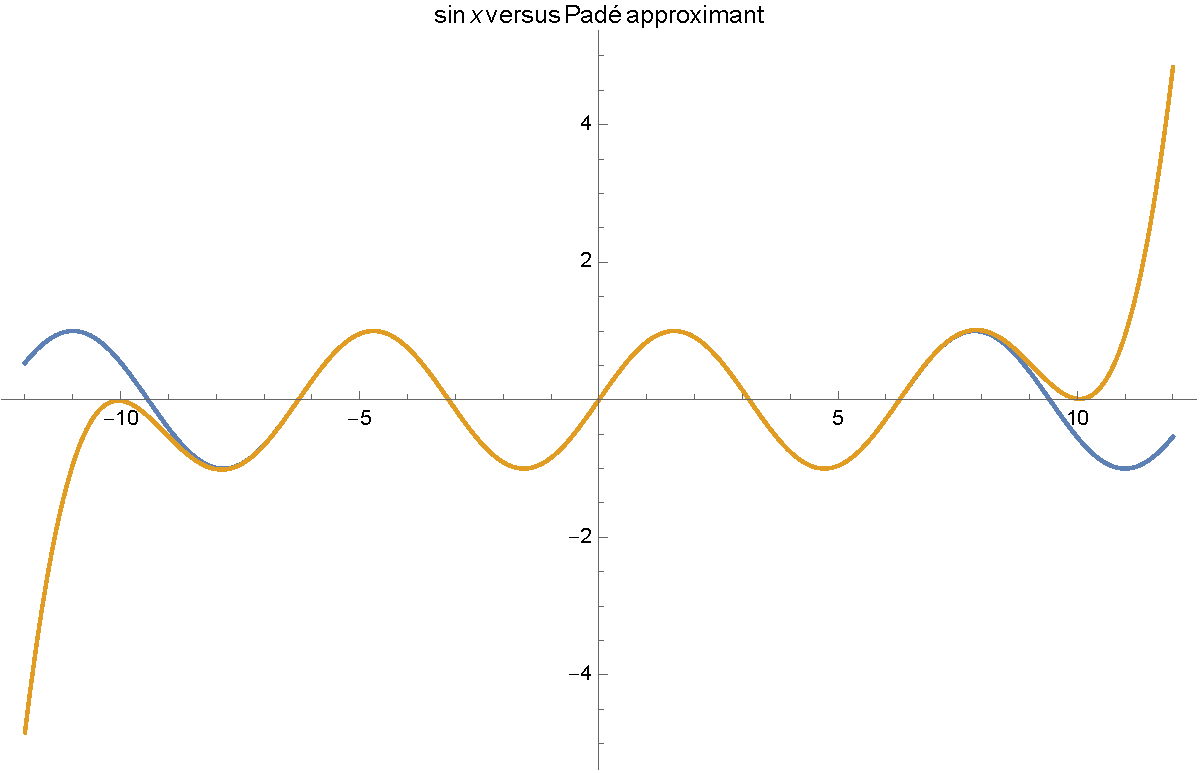
\includegraphics[width=0.75\textwidth]{Pade}
\caption{Comparing $\sin(x)$ with an order $10$ Pad\'e approximant.}\label{pade}
\end{centering}
\end{figure}

%%%%%%%%%%%%%%%%%%%%%%%%%%%%%%%%%%%%%%%%%%%%%%%%%%%%%%%%

\subsection{Tangent}
You will recall that $\tan(x) = {\sin(x)} / {\cos(x)}$ but
that it is undefined when $\cos(x) = 0$, that is when $x$ is a
multiple of ${\pi}/{2}$. You \emph{could} just do the division:
\begin{lstlisting}
double tan(double x) { return sin(x) / cos(x); }
\end{lstlisting}

While doing the division is correct in the \emph{real numbers},
remember that we are working with \emph{approximations} and so you will
be more accurate with a formula for directly computing your approximation
for $\tan(x)$.  A Pad\'e approximant for $\tan(x)$ is:
$$
\tan(x)\approx
\frac{x \left(x^8-990 x^6+135135 x^4-4729725 x^2+34459425\right)}{45 \left(x^8-308
   x^6+21021 x^4-360360 x^2+765765\right)} .
$$
\textcolor{red}{You will want to rewrite it in Horner normal form before using it.}
%%%%%%%%%%%%%%%%%%%%%%%%%%%%%%%%%%%%%%%%%%%%%%%%%%%%%%%%

\subsection{\Large $e^x$}
The other important function is $e^x$ called the \emph{exponential}
function.  While you might hope for a Pad\'e approximant, you are
bound for disappointment.  The domain of $e^x$ is unrestricted so
we will \emph{not} be able to use any fixed formula.  As we get further
away from where we center our series, the more terms that will need
to get good results. Fortunately, the series for $e^x$ converges
very quickly.

Let's consider how well this works. In Figure \ref{exp}, we will
use our expansion to $10$ terms and plot for $e^0 , \ldots  ,
e^{10}$. After about $7$, the approximation starts to diverge
significantly. What this tells us is that $10$ terms is not enough.

\begin{figure}[hbt]
\begin{centering}
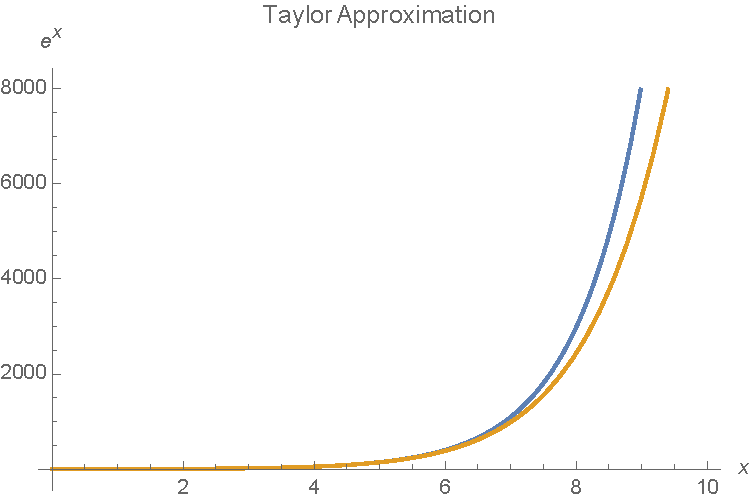
\includegraphics[width=0.75\textwidth]{Exp}
\caption{Comparing $e^x$ with its Taylor approximation centered at zero.}\label{exp}
\end{centering}
\end{figure}


%%%%%%%%%%%%%%%%%%%%%%%%%%%%%%%%%%%%%%%%%%%%%%%%%%%%%%%%
%%%%%%%%%%%%%%%%%%%%%%%%

\begin{figure}[hbt]
\begin{centering}
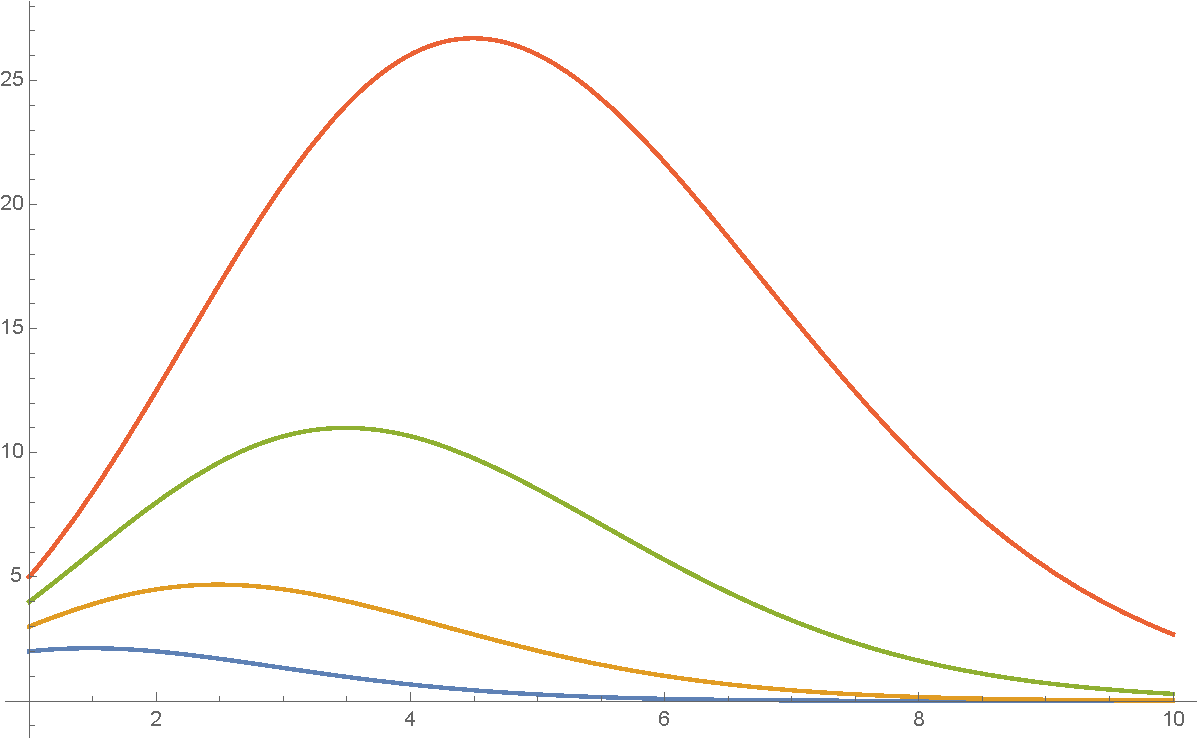
\includegraphics[width=0.75\textwidth]{Growth}
\caption{Comparing ${x^n}/{n!}$ for $x=2,3,4,5$.}\label{growth}
\end{centering}
\end{figure}
%%%%%%%%%%%%%%%%%%%%%%%%%%
If we are na\"ive about computing the terms of the series we can
quickly get into trouble --- the values of $k!$ get large very quickly.
We can do better if we observe that:
$$
\frac{x^n}{n!} = \frac{x^{n-1}}{(n-1)!} \times \frac{x}{n} .
$$

At first, that looks like a recursive definition (and in fact, you
could write it that way, but it would be wasteful). As we progress
through the computation, assume that we know the previous result.
We then just have to compute the next term and multiply it by the
previous term.  At each step we just need to compute ${x} / {n}$,
starting with $n= 0! = 1$ and multiply it by the previous value and
add it into the total.  It turns into a simple \texttt{for} or
\texttt{while} loop.

We can use an $\epsilon$ (epsilon) to halt the computation since
$|x^n| < n!$ for a sufficiently large $n$.  Consider Figure \ref{growth}:
briefly, $x^n$ dominates but is quickly overwhelmed by $n!$ and so
the ratio rapidly approaches zero.
\textcolor{red}{For this assignment, $\epsilon = 10^{-9}$ will be sufficient.} \\

\begin{prelab}{Pre-lab Part 1}
  \begin{enumerate}
    \item Write pseudo-code for approximating $e^x$ with either a \textit{for} or
          \textit{while} loop.
    \item Write pseudo-code for printing the output for $e^x$.
  \end{enumerate}
\end{prelab}

\subsection{Command-line Arguments}
Your program will use command-line arguments to select which one of your
implemented functions to run. You will use \texttt{getopt()} to parse
command-line arguments, which is included under \texttt{getopt.h}. In most
\textbf{C} programs, you will see two parameters in the \texttt{main()}
function: \texttt{int argc} and \texttt{char **argv}. The parameter
\texttt{argc} refers to the argument counter, or how many arguments were
supplied on the command-line. Arguments are delimited by white space, which
includes spaces and tabs.  The parameter \texttt{argv} refers to the argument values, and
is interpreted as an array of strings, where \texttt{argv[0]} corresponds to the
first argument on the command-line: the executable itself.

Try this code, and make sure that you understand it:
\begin{lstlisting}
#include <stdio.h>

int main(int argc, char **argv) {
  for (int i = 0; i < argc; i += 1) {
    printf("argv[%d] = %s\n", i, argv[i]);
  }
  return 0;
}
\end{lstlisting}

Command-line options must be defined in order for \texttt{getopt()} to
parse them. These options are defined in a string, where each character in the
string corresponds to an option character that can be specified on the on the
command-line. Upon running the executable,
\texttt{getopt()} scans through the command-line arguments, checking for option
characters.

As an example, the following program supports two command-line options,
`\texttt{p}' and `\texttt{i}'. Note that the option character `\texttt{i}' in the defined option string
\texttt{OPTIONS} has a colon following it. The colon signifies that, when the
`\texttt{i}' option is enabled on the command-line using `\texttt{-i}', \texttt{getopt()} is
looking for an argument to be supplied following it. An error is thrown by
\texttt{getopt()} if an argument for a flag requiring one is not supplied.

\begin{lstlisting}
#include <getopt.h>
#include <stdio.h>
#include <stdbool.h>

#define OPTIONS "pi:"

int main(int argc, char **argv) {
  int c = 0;
  bool print = false;
  char *infile = NULL;

  while ((c = getopt(argc, argv, OPTIONS)) != -1) {
    switch (c) {
    case 'p': // Print option.
      print = true;
      break;
    case 'i': // Input file option.
      infile = optarg;  // A pointer to the next element in argv.
      break;
    }
  }

  if (argc == 1) {
    puts("Error: no arguments supplied!");
    return -1;
  }

  if (!infile) {
    puts("Error: input file required!");
    return -1;
  }

  if (print) {
    puts(infile);
  }

  return 0;
}
\end{lstlisting}

What this program does is check for the `\texttt{p}' option to print and the
`\texttt{i}' option to specify some input file name.
The \texttt{getopt()} defined variable \texttt{optarg} points at the following
\texttt{argv}-element, which in this case should be the input file name. The
condition \texttt{argc == 1} checks if no other command-line arguments were
supplied other than the executable itself and errors out if so. The program also
errors out in the event that an input file name was not supplied. The supplied
input file name is only printed if the print option was specified on the
command-line.

Example usage of program to specify input file and print its name (assume the
executable name is \texttt{filename}):
\begin{lstlisting}
./filename -p -i <input file name>
\end{lstlisting}

Your program \emph{must} support the following command-line options:
\begin{enumerate}
    \item \texttt{-s} : runs \texttt{sin} tests
    \item \texttt{-c} : runs \texttt{cos} tests
    \item \texttt{-t} : runs \texttt{tan} tests
    \item \texttt{-e} : runs \texttt{exp} tests
    \item \texttt{-a} : runs \emph{all} tests
\end{enumerate}

These options are mutually exclusive; only one may be chosen at a time. Is a
\texttt{bool} the best choice, or would an \texttt{enum} be better? \\

\begin{prelab}{Pre-lab Part 2}
  \begin{enumerate}
    \item What does \texttt{getopt()} return? Hint: check the man page.
    \item Is a \texttt{bool} or an \texttt{enum} the best choice? Explain why.
    \item Provide pseudo-code for your main function. Assume you have helper functions
          available to you.
  \end{enumerate}
\end{prelab}

% \subsection{}
%%%%%%%%%%%%%%%%%%%%%%%%%%%%%%%%%%%%%%%%%%%%%%%%%%%%%%%%

\section{Deliverables}
\epigraph{\emph{Thinking doesn't guarantee that we won't make mistakes. But
not thinking guarantees that we will.}}{---Leslie Lamport}

\noindent You will need to turn in:

\begin{enumerate}
  \item \texttt{math.c}: This is your main program that determines whether
      \texttt{exp}, \texttt{sin}, \texttt{cos}, or \texttt{tan} will be run as
      well as contain your implementations. \texttt{getopt()} must be used to
      handle command-line arguments dictating which tests to run.
        The \texttt{getopt()} options you must support are
        `\texttt{-s}' to run \texttt{sin} tests, `\texttt{-c}' to run
        \texttt{cos} tests, `\texttt{-t}' to run \texttt{tan} tests,
        `\texttt{e}' to run \texttt{exp} tests, and `\texttt{-a}' to run
        \emph{all} tests. Your output for each function must match the form
        shown in Figures \ref{sine} and \ref{cosine}.
        Your compiled program must be called \texttt{math}.

  \item \texttt{Makefile}: This is a file that will allow the grader to type
      \texttt{make} to compile your program. Typing \texttt{make} must build
        your program and running \texttt{./math} alone as well as with option flags must run your program.
  \begin{itemize}
    \item \texttt{CFLAGS=-Wall -Wextra -Werror -Wpedantic} must be included.
    \item \texttt{CC=clang} must be specified.
    \item \texttt{make clean} must remove all files that are compiler generated.
    \item \texttt{make infer} must run \texttt{infer} on your program.
        Complaints generated by \texttt{infer} should either be fixed or
        explained in your \texttt{README}.
    \item \texttt{make} should build your program, as should \texttt{make all}.
  \end{itemize}

  \item \texttt{README.md}: This must be in \emph{markdown}. This
      must describe how to use your program and \texttt{Makefile}. This is also
      where you put any explanations for complaints generated by \texttt{infer}.

  \item \texttt{DESIGN.pdf}: This \emph{must} be a PDF. The design document
  should contain answers to the pre-lab in the beginning and describe your design
  for your program with enough detail that a sufficiently knowledgeable programmer
  would be able to replicate your implementation. This does not mean copying your
  entire program in verbatim. You should instead describe how your
  program works with supporting pseudo-code. For this assignment pay extra attention to how
  you describe your representation of a Taylor series approximation in \textbf{C}.
  You \emph{must} push the DESIGN.pdf before you push \textcolor{red}{\emph{any}} code.

  \item \texttt{WRITEUP.pdf}: This \emph{must} be a PDF. Your WRITEUP should be a discussion of the results for your
  experiments. This means analyzing the differences in the output of
  your implementations versus those in the \texttt{math.h} library.
  Include possible reasons for the differences between your implementation
  and the \texttt{math.h} version. Graphs can be especially useful
  in showing the differences and backing up your arguments.

\end{enumerate}


%%%%%%%%%%%%%%%%%%%%%%%%%%%%%%%%%%%%%%%%%%%%%%%%%%%%%%%%

\section{Submission}
\epigraph{\emph{We in science are spoiled by the success of mathematics.
Mathematics is the study of problems so simple that they have good
solutions.}}{---Whitfield Diffie}

To submit your assignment, refer back to \texttt{asgn0} for the steps on how to submit your assignment through \texttt{git}. Remember: \emph{add, commit,} and \emph{push}!

\textcolor{red}{Your assignment is turned in \emph{only} after you have pushed.
If you forget to push, you have not turned in your assignment and you will get
a \emph{zero}. ``I forgot to push'' is not a valid excuse. It is \emph{highly} recommended to commit and push your changes \emph{often}.}

\begin{figure}[ht]
  \centering
    
\includegraphics[width=0.33\textwidth]{../assignment1/obey.jpg}
\end{figure}

%%%%%%%%%%%%%%%%%%%%%%%%%%%%%%%%%%%%%%%%%%%%%%%%%%%%%%%% 
\section{Supplemental Readings} 
\epigraph{\emph{The more that you read, the more things you will know. The 
more that you learn, the more places you'll go.}}{---Dr.\ Seuss}\noindent 
 
\begin{itemize} 
  \item \textit{The C Programming Language} by Kernighan \& Ritchie 
  \begin{itemize} 
    \item Chapter 3 \S 3.4-3.7
    \item Chapter 4 \S 4.1 \& 4.2
    \item Chapter 7 \S 7.2
    \item Appendix B \S B4 
  \end{itemize} 
\end{itemize} 
 
%%%%%%%%%%%%%%%%%%%%%%%%%%%%%%%%%%%%%%%%%%%%%%%%%%%%%%%%%%% 

\end{document}
